% Created 2021-04-16 Fri 10:36
% Intended LaTeX compiler: pdflatex
\documentclass[a4paper]{article}
\usepackage[utf8]{inputenc}
\usepackage[T1]{fontenc}
\usepackage{graphicx}
\usepackage{grffile}
\usepackage{longtable}
\usepackage{wrapfig}
\usepackage{rotating}
\usepackage[normalem]{ulem}
\usepackage{amsmath}
\usepackage{textcomp}
\usepackage{amssymb}
\usepackage{capt-of}
\usepackage{hyperref}
\usepackage{listingsutf8}
\usepackage{minted}
\usepackage[margin=0.5in]{geometry}
\usepackage{parskip}
\author{Marco Hassan}
\date{\today}
\title{Literature Review}
\hypersetup{
 pdfauthor={Marco Hassan},
 pdftitle={Literature Review},
 pdfkeywords={},
 pdfsubject={},
 pdfcreator={Emacs 27.1.91 (Org mode 9.4.4)}, 
 pdflang={English}}
\begin{document}

\maketitle
\tableofcontents

\setlength\parindent{0pt}
\newpage

\section{Scope}
\label{sec:org9b655b0}

This file summarizes some interesting literature that is important
to consider for your work.

You can write down here some papers with major ideas.


\section{Literature Review}
\label{sec:org69d442e}

\subsection{Mrad et all - On the types of Uncertainty}
\label{sec:orgc4a519e}
\begin{itemize}
\item \cite{Mrad_2015}
\end{itemize}

Literature review. Say that the distinction among the different
types of evidence is not clear.

Three types of \emph{uncertain evidence}:

\begin{itemize}
\item likelihood evidence
\item fixed probabilistic evidence
\item non-fixed probabilistic evidence
\end{itemize}

The authors state that often it is not clear the difference among
the three and they are not treated well enough. I.e. many engines
and frameworks do not make such distinctions well enough so that
you do not account for the difference among the three when doing
propagation work.

General loop in inference:

\begin{center}
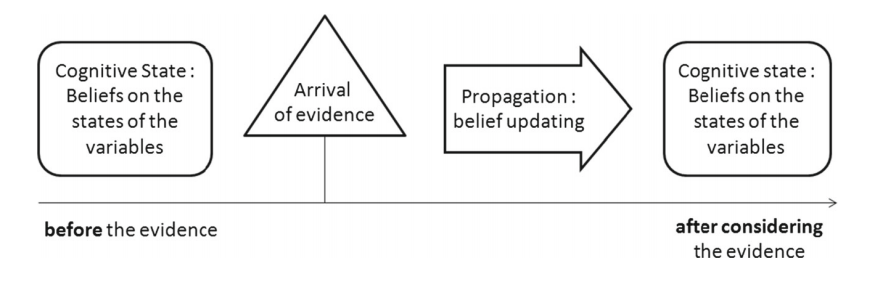
\includegraphics[width=.9\linewidth]{/Users/marcohassan/Desktop/Bayesian_Net_Thesis/images/inference_loop.png}
\end{center}

\subsubsection{In table 1 different papers that were dealing with Likelihood evidence at inference time.}
\label{sec:orgab35411}


\subsubsection{Definitions}
\label{sec:org0641c15}

Nice \textbf{definition of Bayesian Networks}:

\begin{quote}
Bayesian networks are probabilistic graphical models that provide a
powerful way to embed knowledge and to update one’s beliefs about
target variables given new information about other variables./
\end{quote}

On \textbf{evidence}:

\begin{quote}
A piece of evidence is also called a finding or an observation, and
evidence refers to a set of findings.
\end{quote}

\textbf{Definition Variable Instantiation:}

\begin{quote}
A finding on a variable commonly refers to an instantiation of the
variable.  This can be represented by a vector with one element
equal to 1, corresponding to the state the variable is in, and all
other elements equal to zero. This type of evidence is usually
referred to as \textbf{hard evidence} though other terms are sometimes used.
\end{quote}

Note that hard fininding/evidence = observation.

\textbf{Definition Uncertain Evidence:}

\begin{quote}
This paper focuses on another type of evidence that cannot be
represented by such vectors: uncertain evidence
\end{quote}


\textbf{Definition Likelihood Evidence:}

\begin{quote}
Likelihood evidence is applicable when there is uncertainty about the
veracity of an observation, such as, for example, the information
given by an imperfect sensor
\end{quote}

\textbf{Definition Probabilistic Evidence:}

\begin{quote}
In contrast probabilistic evidence can be regarded as a \textbf{new
probability distribution} on a variable arising from a new
observation after creation of the model. This is dissimilar to
likelihood evidence where the \textbf{original probability distribution is
not challenged}, only ones belief in it and which may be amended
with new likelihood evidence.
\end{quote}


\subsubsection{Two possibilities for uncertain input}
\label{sec:orge54378f}

\begin{enumerate}
\item the uncertainty bears on the meaning of the input; the
existence of the input itself is uncertain, due to, for
instance, the \emph{unreliability of the source that supplies
inputs}

\item the input is a partial description of a probability measure
\end{enumerate}


\subsubsection{Likelihood Evidence}
\label{sec:org1a7cef8}

Here observation is uncertain due to unreliable source of
information. We are in case 1. above.

This is clear. You got it and is straightforward.

Here the observation itself \textbf{is} uncertain.

Likelihood evidence / findings are defined as follows:

\begin{center}
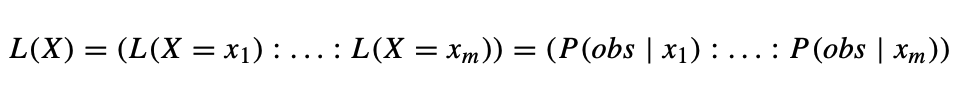
\includegraphics[width=.9\linewidth]{/Users/marcohassan/Desktop/Bayesian_Net_Thesis/images/Bildschirmfoto_2021-03-22_um_17.42.33.png}
\end{center}


\textbf{Weird image; normalized or not? Cause there does not seem to be
any evidence in there.}

Note therefore that the probability is not assigned as P (x\textsubscript{i} |
evidence) but rather the contrary. Watch out to this as I guess
that you interpreted it in the wrong way so far.

\textbf{Note} likelihood evidence is specified \emph{without a prior}. As a
consequence, propagating likelihood evidence takes into account
the \textbf{beliefs in the variable}  before the evidence. 

I.e. you propagate based on the likelihood not based on evidence.

To understand this read the following and check example 1.

\textbf{important} what follows is key to be inserted in the literature
review. The likelihood evidence \textbf{does not incorporate} any prior
knowledge. See example 1 in the paper. I.e. it is ment to be seen
as an \emph{external application that delivers the likelihood of a
variable realization}.  It does not account however the
probabilistic structure implied by the model.

Note also that the sum of the above likelihood ratios does not
have to sum to 1 so it is not a probability metric.

The key takeway is:

\begin{quote}
In order to update the belief in the value of the character, the
information provided by the OCR (the vector of similarity) has to be
combined with the prior knowledge about the frequency of
letters. Moreover, the result of propagation is not fixed since belief
in X can be further modified by other information.

For example you can leverage information about the adjacent characters.
\end{quote}


\subsubsection{Probabilistic evidence.}
\label{sec:orgf01b4ae}

This encompasses uncertain evidence specified by a local
probability distribution.

It can be broken down into two further sub-categories.

\begin{itemize}
\item fixed probabilistic evidence <=> soft evidence as in \cite{Valtorta_2002}.

\item not-fixed probabilistic evidence
\end{itemize}

Note that the terms \emph{fixed} and \emph{non-fixed} capture the expected
behavior of the posterior probability after further evidence is
obtained.

Recall that in \texttt{likelihood evidence} we said that the sum of the
entries does not sum to 1 and \textbf{does not represent in this sense
any local probability structure as it does not consider the structure of the network}.

In contrast in \emph{probabilistic evidence} there is another meaning
of uncertain input. Here in fact the evidence is specified by a
\textbf{local probability} distribution. This no matter if we are talking
about \emph{fixed} or \emph{non-fixed} probabilistic evidence. \textbf{Both are
ultimately} probabilistic evidences.

So this is basically it and the definition goes as follows:

\begin{quote}
A probabilistic finding on a variable X ∈ X is specified by a local
probability distribution R(X) that defines a constraint on the belief
in X after this information has been propagated; it describes the
state of beliefs in the variable X “all things considered”. A
probabilistic finding is fixed (or not) when the distribution R(X) can
not be (or can be) modified by the propagation of other
findings. Probabilistic evidence is a set of probabilistic findings.
\end{quote}

So you understand that the conditioning on other variables makes
the difference.

\textbf{Note the following when propagating:} 3 A probabilistic finding
R(X) on a variable X of a Bayesian network \textbf{replaces any prior
belief or knowledge on X}. As a consequence, the prior P (X) is not
used in the propagation of R(X), and any previous finding or
belief on X is lost.

So the idea is that an expert call can overwrite any prior
belief. [[\label{question-where-does-the-probabilistic-finding-come-from}

Note the following definition. This will be key to understand
fixed vs. non-fixed probabilistic evidence. In fact the meat is
all there.

\begin{center}
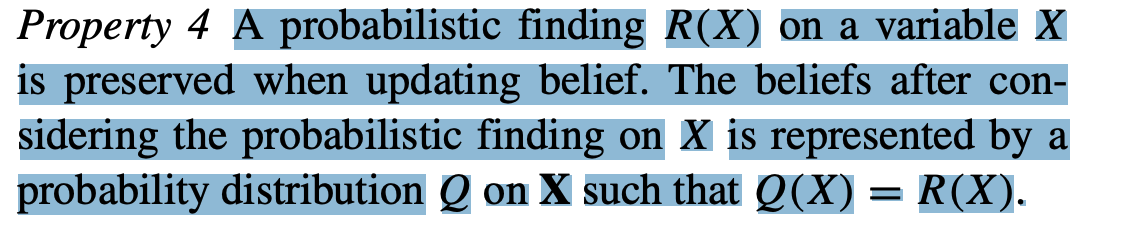
\includegraphics[width=.9\linewidth]{/Users/marcohassan/Desktop/Bayesian_Net_Thesis/images/Bildschirmfoto_2021-03-26_um_12.14.27.png}
\end{center}


Note that the last equality holds in the case of fixed
probabilistic evidence. This is in fact the key result.

Note that as mentioned a couple of times already \emph{fixed-evidence}
implies that we do not alter Q(X) when propagating new evidence (in
all cases where the evidence does come to X, i.e for all variables
but this). 

This means that any kind of evidence received on other variables after fixed
probabilistic evidence makes it necessary to re-propagate previous
fixed probabilistic evidence together with the new evidence, in
order to keep the former probabilistic evidence fixed.

\begin{quote}
Fixed probabilistic evidence behaves as hard evidence in that the
specified evidence remains unchanged after its propagation, and still
remains unchanged after the arrival of other information on the same
case.
\end{quote}

\begin{quote}
\textbf{Definition:} A not-fixed probabilistic finding on X can be
modified by further evidence on \textbf{any variable} in the model
\end{quote}

To make sense about such fixed and non-fixed probabilistic
evidence you can check at the examples in the paper. (ex 3 -
4). It is pretty much straightforward the concept when you look at
it in simple examples. People should be more to the point at
times.

\textbf{Note} important that in order to be considered \emph{fixed
probabilistic} findings you usually require that the R(X) is given
with the property of \emph{all things considered}, i.e. considering all
of the variables in the network. In such a way even if new
evidence arrives in the network it does not affect R(X) when
making inference as the information is already included in the
probabilistic fixed evidence.

Note that you can think of fixed probabilistic evidence as a
constraint on the posterior probability.


\subsubsection{On the big difference among likelihood and evidence}
\label{sec:org661372d}


\begin{enumerate}
\item for probabilistic evidence the distribution is specified “all
things considered” whereas for likelihood evidence the
likelihood ratio is without prior knowledge or belief

\item propagation: while probabilistic evidence remains unchanged by
updating the observed variables, likelihood evidence has to be
combined with previous beliefs in order to update the belief in
the observed variable(s).
\end{enumerate}

So these two are the major differences and you can think in the
next couple of days how you can integrate your algorithm to deal
with such type of evidence.


\subsubsection{Interesting concept extended probabilistic finding.}
\label{sec:org87c2ef7}

This is defined as follows:

\begin{center}
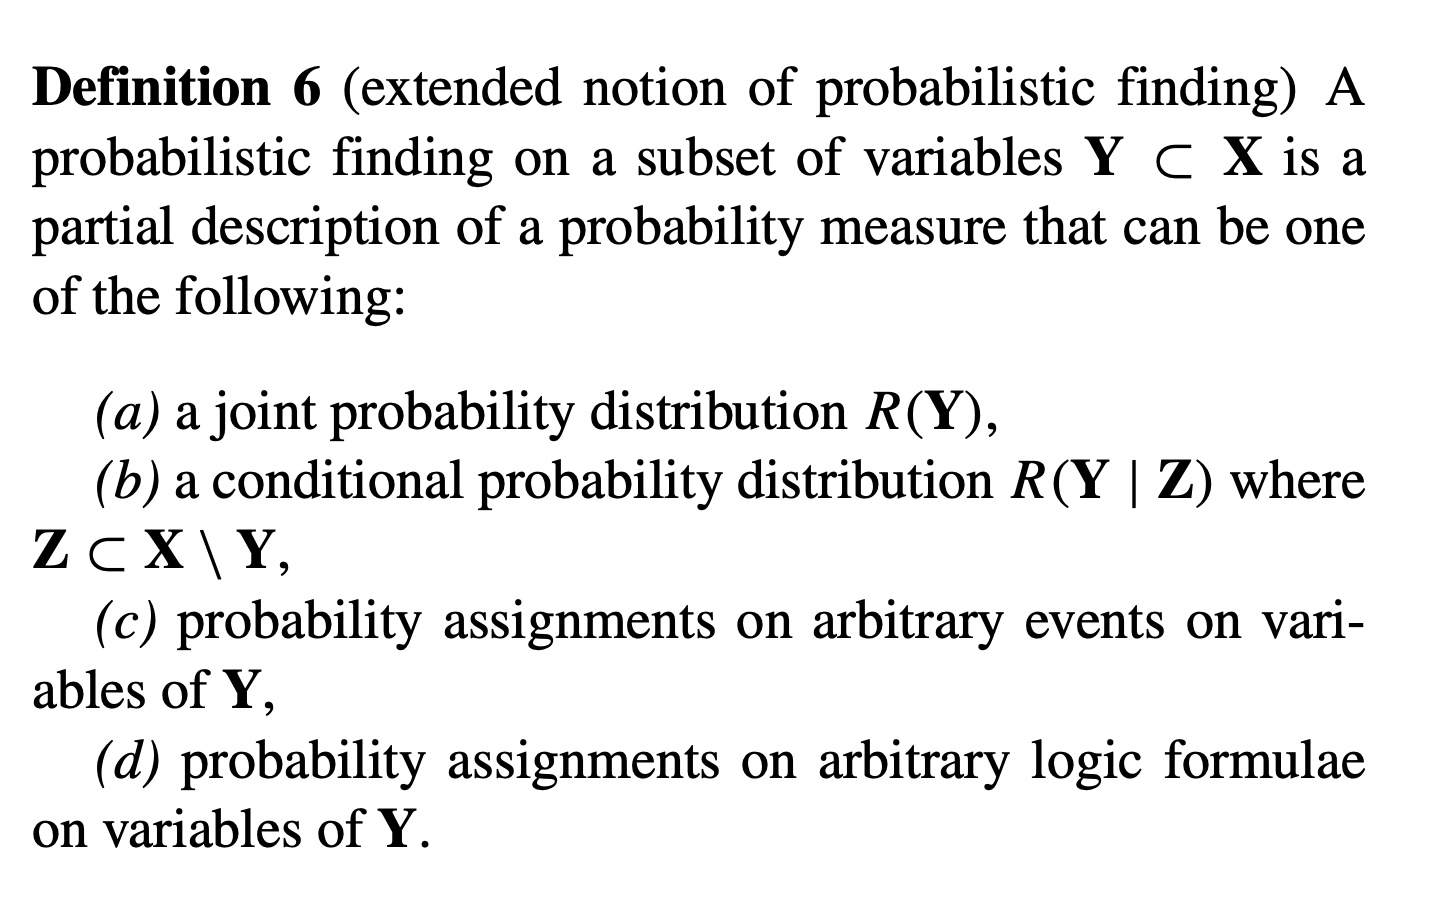
\includegraphics[width=.9\linewidth]{/Users/marcohassan/Desktop/Bayesian_Net_Thesis/images/Bildschirmfoto_2021-03-26_um_16.41.09.png}
\end{center}


Given such definition it is then written in the paper that:

\begin{quote}
The extended notion of probabilistic evidence can be handled for
evidence updating by the introduction of an observation node
[69]. This technique allows the reformulation of extended
probabilistic evidence into probabilistic evidence on a single new
observation variable.
\end{quote}

i.e. check this paper 69 cause this is in fact very similar to
what was done in your case.



\subsubsection{On propagation of likelihood and probabilistic evidence}
\label{sec:org7d7a9a8}

Here the paper discusses the two separately.

On the one hand you deal with propagation of likelihood via the
method of Pearl often encountered and discussed in the paper.

On the other hand you use Jeffery's method to deal with
propagation in the case of probabilistic evidence.

\begin{enumerate}
\item Pearl's Method
\label{sec:orgcbe4e73}

Virtual evidence refers to Pearl’s idea of interpreting a
likelihood finding on an event \textbf{as a hard finding on some virtual
event that only depends on this event} [61]. The virtual evidence
method provides a convenient way of incorporating evidence with
uncertainty in a Bayesian network.

I.e. this is the idea you extend the network with a virtual node
and you assign a hard finding to it and state that the
probability of such hard finding is defined by the likelihood
ratios.

The hard evidence on the added node is propagated using a
classical inference algorithm in the Bayesian network.

So recall now that the likelihood evidence entries given L(X) in
express the following condition P(o | X). For the posterior after
propagating we are interested in Q(X) = P(X |O = o) or consistent
with the notation of Koller and Friedman P(X | E = e).

Where the P(X | O = o) depends on the following:

\begin{center}
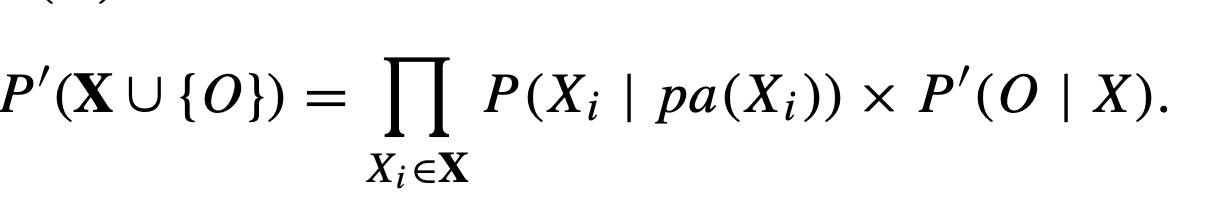
\includegraphics[width=.9\linewidth]{/Users/marcohassan/Desktop/Bayesian_Net_Thesis/images/Bildschirmfoto_2021-03-26_um_17.12.45.png}
\end{center}

It should now immediately be clear the property discussed
before - i.e. that the posterior in the case of the likelihood
\textbf{depends on the prior belief in X} and has in fact to bbe
combined with that and propagated in order to come to the
posterior.

\item Jeffery's Method
\label{sec:org2fd954c}

Here we are again interested in propagating in the bayesian
network and ultimately get the posterior probability for P(X |
evidence).

The issue here is that for such a model when we propagate and
compute the posterior we must consider the local probability
distribution R(X) and its implications - i.e. how this will be
updated. I.e. we cannot blindly compute the posterior but we
rather have to understand how the information flows in the
network and influences R(X). 


The issue moreover is that we cannot treat R(X) as a
hard-evidence and then propagate keeping such constraint as R(X)
is in fact \textbf{not a hard evidence} but rather is a probabilistic
evidence representing a CPD . So we need a way to come up with
hard-evidence or something similar as done by the method of
Pearl in order then to propagate. I.e. we have to deal with such
condition. (cite and look at 64)

Moreover it follows that

A probabilistic finding R(X) requires a \textbf{reconsideration of the
joint probability distribution P} because it replaces the existing
prior on the variable X. (and recall that the joint is
\emph{conditional * prior}.

I.e.

\begin{quote}
The propagation of probabilistic evidence requires the
replacement of the initial probability distribution P by
another probability distribution Q that reflects the beliefs in
the variables of the model after accepting the probabilistic
evidence.
\end{quote}

This replacement is not definitive: it lasts as long as the
specific observed case holds.

Jeffrey’s approach for this problem is known as “probability
kinematics” and it is based on the following points:

\begin{itemize}
\item The posterior probability distribution on the observed variable
X Q(X) is unchanged: Q(X) = R(X),

\item conditional probability distribution of other variables given X
remains invariant under the observation: Q(X $\backslash$ \{X\} | X) = P (X
$\backslash$ \{X\} | X).

\item It follows then the following Jeffery's Rule:

\begin{center}
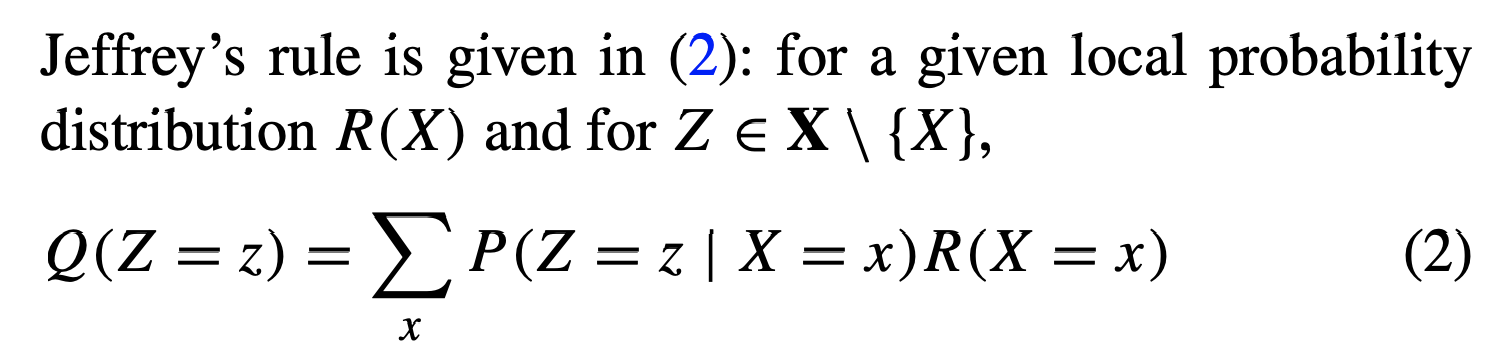
\includegraphics[width=.9\linewidth]{/Users/marcohassan/Desktop/Bayesian_Net_Thesis/images/Bildschirmfoto_2021-03-26_um_18.04.54.png}
\end{center}

This is how you define the CPD of each variables and from there
you can finally compute the joint.

\textbf{Note the following!!}

\begin{center}
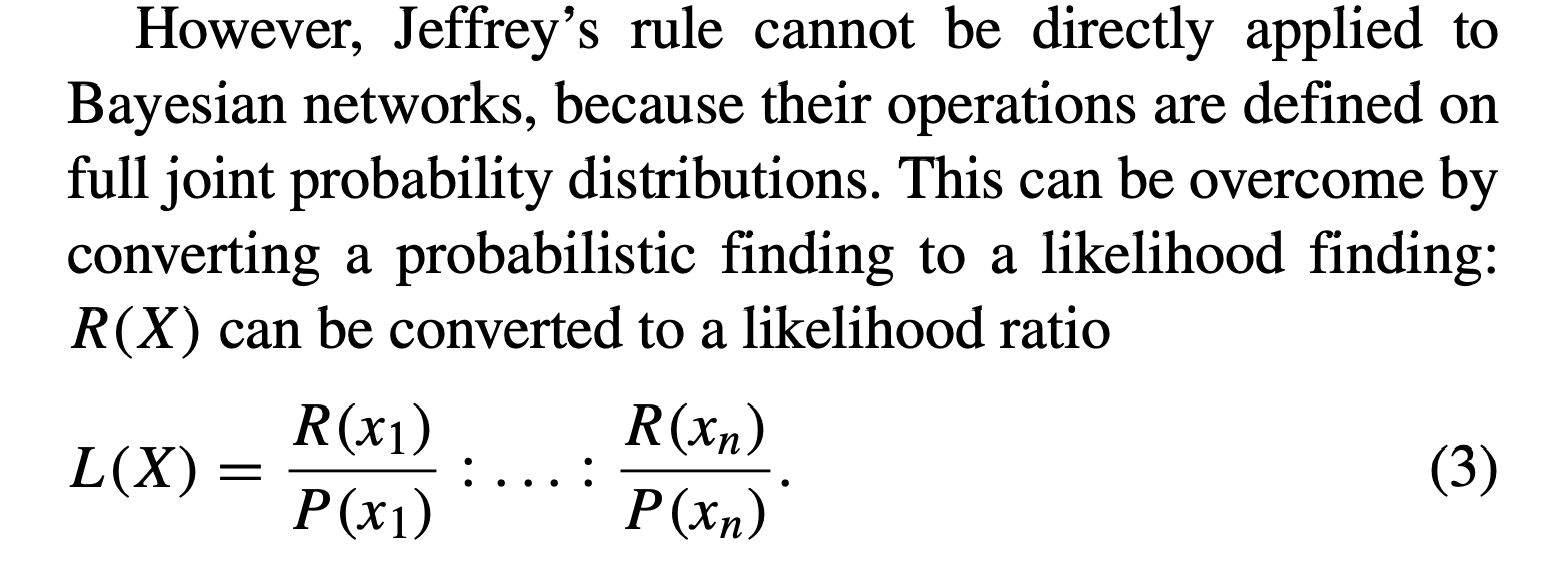
\includegraphics[width=.9\linewidth]{/Users/marcohassan/Desktop/Bayesian_Net_Thesis/images/Bildschirmfoto_2021-03-26_um_18.07.55.png}
\end{center}

Understand it cause also here it seems that everything is
pretty straightforward and extendible as there is a clear
pipeline:

probabilistic evidence -> likelihood evidence -> hard evidence.

And so then you can maybe apply the same algorithm there.

Check this ratio might be bigger than 1?

Note that in the conclusion it is written that you apply such a
method to \emph{non-fixed} probabilistic evidence. For the case of
\emph{fixed} probabilistic evidence you work in a different way
using constrained algorithms as discussed in the next section. 

Propagating this likelihood finding L(X) with Pearl’s method
provides the same results as propagating R(X) by Jeffrey’s
rule.

In case of \textbf{several probabilistic findings}, the method of
converting probabilistic findings into likelihood findings does
not preserve probabilistic findings. A simple example can be
found in [15, 64]. --> this because it is immediate to see that
the jeffery's condition are violated. Then Q(X1) != R1(X1) or
Q(X2) != R2(X2) depending on the order of propagation.

It therefore holds that the inclusion of several pieces of
probabilistic evidence with Jeffrey’s rule \textbf{does not commute}. In
other words, final beliefs \textbf{depend on the order of arrival of the
probabilistic findings}.
\end{itemize}


The next section deals with the propagation of several pieces
of fixed probabilistic findings, such that their order does not
modify the final belief.

\item Dealing with several pieces of probabilistic evidence
\label{sec:orgb29c8f0}

\emph{Iterative Proportional Fitting Procedure (IPFP) algorithm}, which
is an iterative method of revising a probability distribution to
respect a set of given probability constraints in the form of
posterior marginal probability distributions over a subset of
variables.

I think this is in fact what the paper I mentioned in the
research proposal deals with: \cite{Masegosa_2016}.

However, the IPFP works on full joint distributions, and thus is
not directly applicable to belief update in Bayesian
networks. Too big network for this. infeasible for larger ones
since it needs to literally modify each entry of the joint
probability distribution table at each iteration.

Solution use \emph{big clique algorithm} is a variation of the
junction tree algorithm.
\end{enumerate}


\subsubsection{Nice debate to include: change model or propagate probabilistic evidence as discussed so far?}
\label{sec:org18ae87f}

\begin{center}
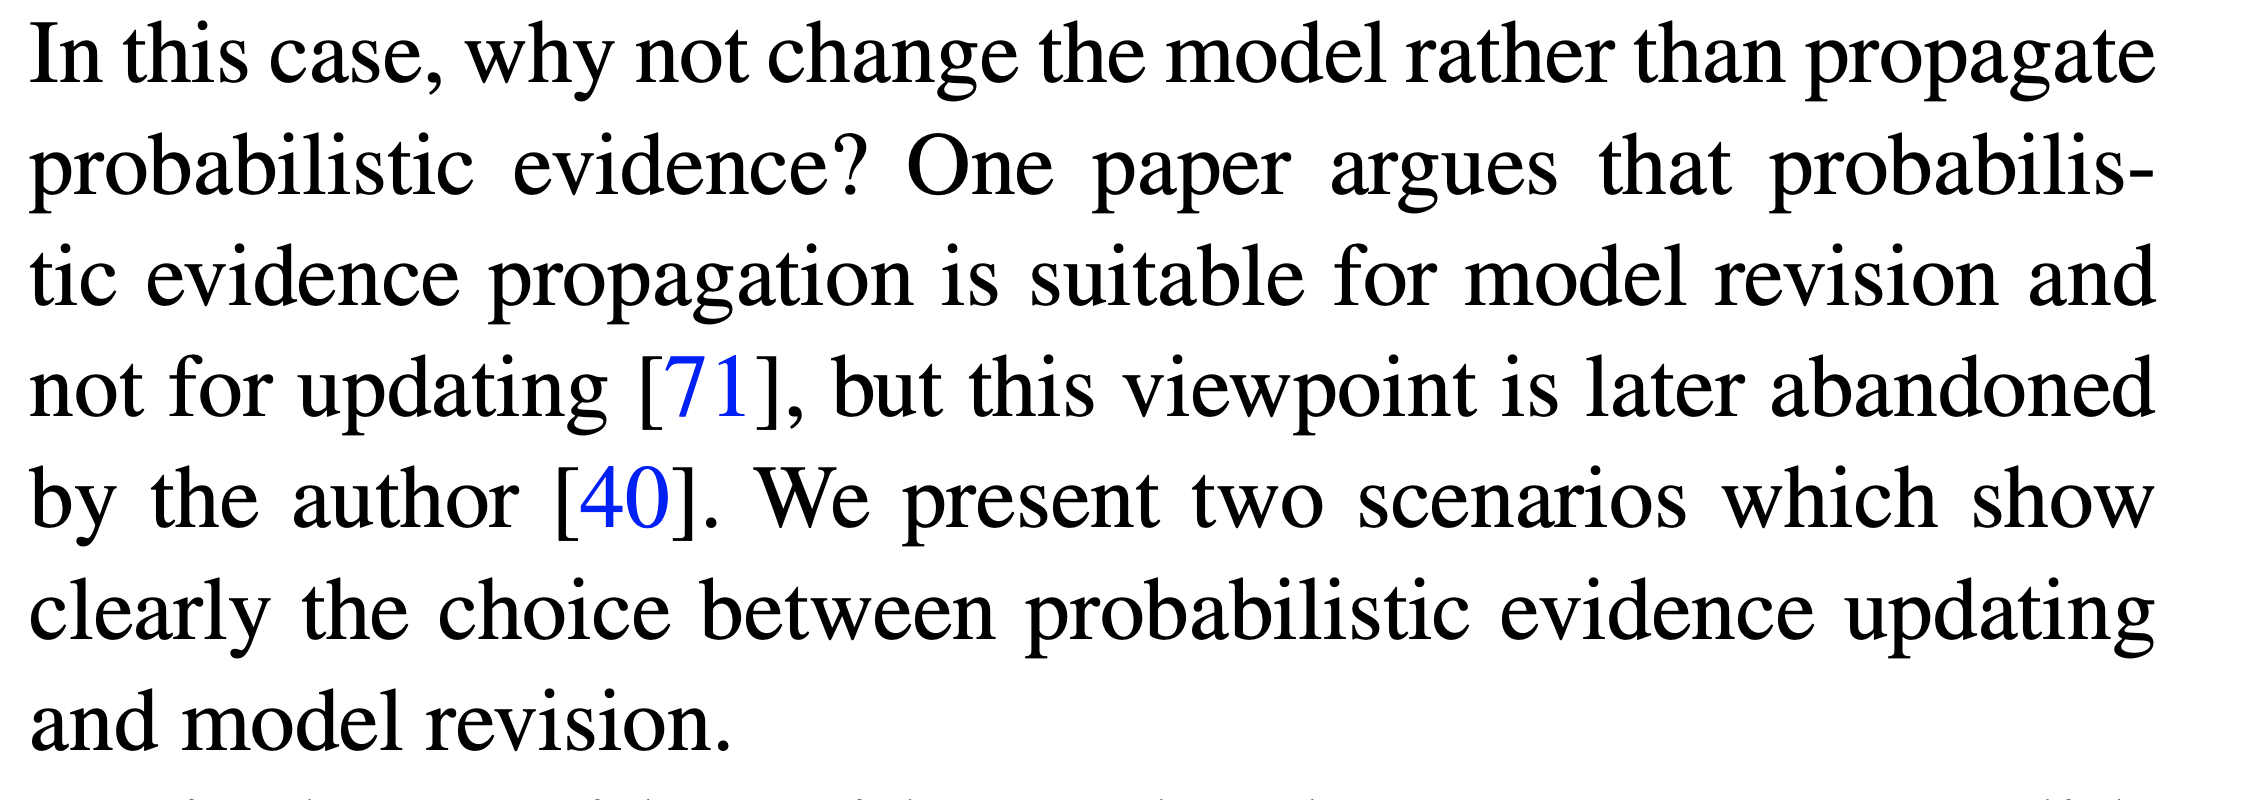
\includegraphics[width=.9\linewidth]{/Users/marcohassan/Desktop/Bayesian_Net_Thesis/images/Bildschirmfoto_2021-03-26_um_19.19.24.png}
\end{center}


Would maybe be nice to include this in the thesis discussion.


\subsubsection{ISSUE}
\label{sec:org926ad6f}

\label{issue_have-still-to-understand-why-propagation-is-necessary}
If it is at the end of the network - say in one leaf then
such propagation might not be needed. If not then I see the
point. Make such reasonings and make them more explicit at some
point when you will have the time.




\subsection{Cite For np-hard problem of exact and approximate inference methods:}
\label{sec:orgf4d0db3}

\cite{Dagum_1993,Cooper_1990}


\subsection{Masegosa 2016 - learning from incomplete data with qualitative influences}
\label{sec:orge9fb8d7}

I think that this is one type of probabilistic evidence as
discussed in Mrad et all.

No actually it is not. It is rather another different type of
evidence. You neither specify a likelihood evidence nor you specify
an "all things considered" conditional probability density.

You rather have an expert setting some constraints of the form this
influence must be bigger than x. Or this increases or decreases the
probability \emph{on that}.

So you would actually have to learn parameters that respects such
constraints. If you move in the space of the MLE after properly
defining the likelihood the problem is simply the one of a
constrained maximization problem that you can solve with the usual
Lagrange multiplier technique. In the case of the EM you just have
to check if the properties apply. If they do then you are more less
set.

This paper takes a different approach. Instead of working with
Lagrange multipliers they augment the EM to respect the various
constraints.

The two algorithms they mention are:

\begin{enumerate}
\item \emph{isotonic regression EM:}

\item \emph{qirEM} builds upon the isotonic regression by reducing the
computational burden.
\end{enumerate}

The essential idea is that \emph{isotonic regression} produces the
constrained MLE without having to go through constraints themselves
explicitly. 

\begin{quote}
Such that as a bottom line you can use the following:

We propose to augment the maximization step of the EM algorithm
with the isotonic regression in order to obtain parameter estimates
that satisfy the order constraints from incomplete data. This
algorithm, called irEM, requires the application of the isotonic
regression in each iteration of EM.
\end{quote}

Qir tries to reduce the computational complexity by applying the
isotonic regression step just one time after convergence. What are
the guarantees of all of that then?

Note however that to achieve this Qir needs convex optimization in
the M-step. Due to the acceptance of just qualitative influences
such optimization can be done in polynomial time.

2.1 defines the problem with missing evidence as in the
book. Pretty 1:1 and nothing new. You sum over all possible
completions.

2.2 also standard results of friedman and koller.

\emph{Definition - Partially Ordered Set:} -> is used to understand
isotonic regression. Ok so nothing special. it is just a set of
relations \emph{smaller\textsubscript{equal}} or \emph{greater\textsubscript{equal}} that completely order
your set.

Definition of isotonic regression is then the following:

\begin{center}
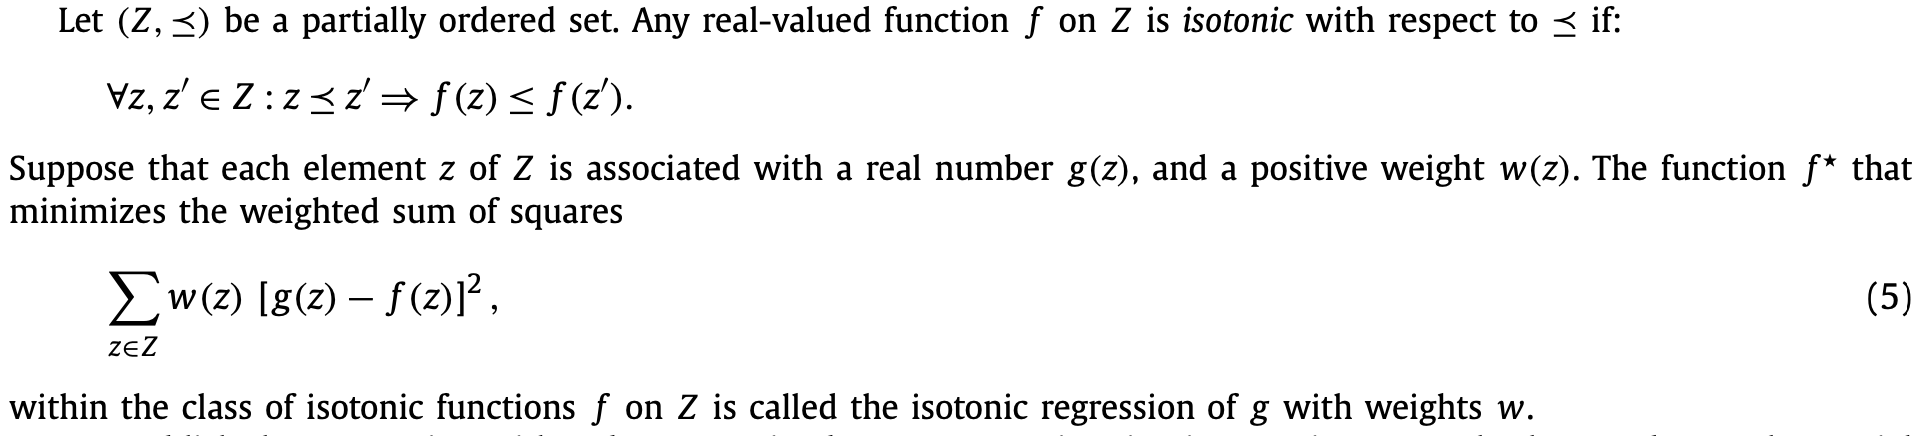
\includegraphics[width=.9\linewidth]{/Users/marcohassan/Desktop/Bayesian_Net_Thesis/images/Bildschirmfoto_2021-03-27_um_18.36.31.png}
\end{center}

Note that f\textsuperscript{*} should be inserted in place of f(z) above and then
you should minimize this.

Check then at the example in the paper to understand how this
partial order translates to the case of a Bayesian network. Nothing
wild. Just have to keep track a bit of notation.

Then basically the idea for the general MLE with complete data is
to leverage the global decomposition property.

Very easy irAlg then you just simply take the isotonic regression
from the respective CPT parameters. You just have to make more
explicit such link of the parameters and read about it once more
the relation with the partial order.

Once this is done everything is pretty much straightforward. You
just do an isotonic regression over this.


\subsection{ISSUEs tracker}
\label{sec:org6e9391d}

\ref{issue_have-still-to-understand-why-propagation-is-necessary}

\ref{question-where-does-the-probabilistic-finding-come-from}

\newpage

\bibliography{references}
\bibliographystyle{unsrt}
\end{document}
